% OPSS Preliminary Design Review — Software Architecture
% Compile with: pdflatex pdr_software_architecture.tex
\documentclass[11pt, letterpaper]{article}

\usepackage[margin=1in]{geometry}
\usepackage{tikz}
\usetikzlibrary{arrows.meta, positioning, fit, backgrounds, calc, shapes.geometric}
\usepackage{amsmath, amssymb}
\usepackage{booktabs}
\usepackage{enumitem}
\usepackage{hyperref}
\usepackage{caption}
\usepackage{xcolor}
\usepackage{fancyhdr}

% ── Color palette ──
\definecolor{sensing}{HTML}{4A90D9}
\definecolor{vision}{HTML}{E67E22}
\definecolor{estimation}{HTML}{27AE60}
\definecolor{validation}{HTML}{8E44AD}
\definecolor{output}{HTML}{C0392B}
\definecolor{infra}{HTML}{7F8C8D}
\definecolor{threadbg}{HTML}{F5F5F5}

% ── Header ──
\pagestyle{fancy}
\fancyhf{}
\lhead{OPSS --- Preliminary Design Review}
\rhead{Software Architecture}
\cfoot{\thepage}

\title{%
  \textbf{Optical Projectile Sensing System (OPSS)}\\[0.3em]
  \Large Preliminary Design Review:\\
  Software Design and Architecture%
}
\author{Autonomous Flight and Perception Laboratory}
\date{\today}

\begin{document}
\maketitle
\thispagestyle{fancy}

% ====================================================================
\section{Software System Overview}
% ====================================================================

The Optical Projectile Sensing System (OPSS) is a real-time perception
and tracking pipeline designed to detect airborne objects using a
stereo depth camera, estimate their three-dimensional state, validate
those estimates against physical constraints, and broadcast the
resulting state to external consumers.  The software architecture is
organized as a modular, staged pipeline that separates sensing,
perception, state estimation, physics validation, fusion, and output
interfaces.  This separation enables independent development and
testing of individual subsystems while maintaining a deterministic
end-to-end execution path.

At runtime, OPSS operates as a producer--consumer system composed of
two primary threads (Figure~\ref{fig:threading}).  A \emph{camera
capture thread} acquires synchronized RGB and depth frames from an
Intel RealSense D435 sensor and publishes them into a bounded queue.
A \emph{pipeline processing thread} consumes the most recent available
frame and executes the full perception stack: object detection,
multi-object tracking, physics validation, state fusion,
visualization, and broadcasting.  The pipeline is \textbf{camera-paced}---it
contains no internal timer or sleep---and is designed to prioritize
freshness of data over backlog accumulation by dropping frames under
overload rather than introducing latency.

The software is decomposed into six major subsystems:

\begin{enumerate}[leftmargin=2em, itemsep=4pt]
  \item \textbf{Sensing Layer} ---
        interfaces with the RealSense camera hardware and produces
        synchronized color and depth frames at a configurable rate.

  \item \textbf{Vision Layer} ---
        performs object detection using a neural detector (YOLOv8 Nano)
        on a downsampled image and maps detections back to full
        resolution with associated depth.

  \item \textbf{State Estimation Layer} ---
        tracks detected objects using interchangeable multi-object
        trackers, including a baseline Kalman filter and a
        physics-aware Unscented Kalman Filter augmented with a learned
        neural correction model (UKF-NN).

  \item \textbf{Physics Validation and Fusion Layer} ---
        evaluates estimated trajectories against kinematic constraints
        and adaptively fuses tracker outputs to improve robustness.

  \item \textbf{Output Interface Layer} ---
        provides annotated visualization via a web dashboard and
        broadcasts state estimates to an external robot controller
        over a Unix-domain socket.

  \item \textbf{Simulation and Training Infrastructure} ---
        supports synthetic data generation, estimator training, and
        offline evaluation using the same software interfaces as the
        runtime pipeline.
\end{enumerate}

\noindent
Figure~\ref{fig:arch} illustrates the high-level data flow between
these subsystems.

% ── Figure 1: High-level architecture ──
\begin{figure}[ht]
\centering
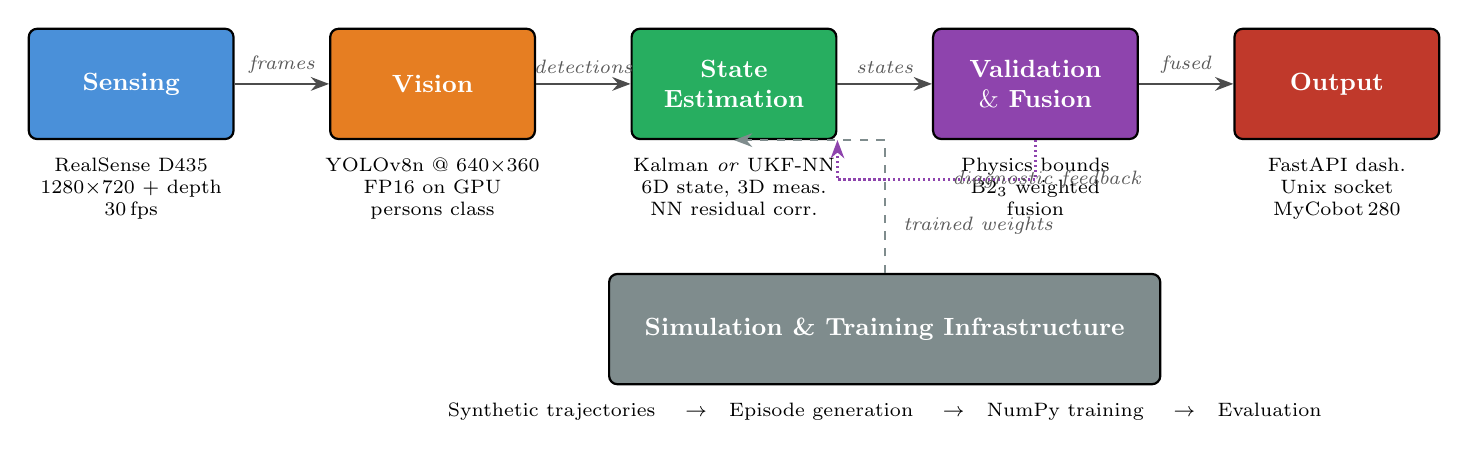
\begin{tikzpicture}[
    >=Stealth,
    node distance=0.6cm and 0.5cm,
    % --- block styles ---
    stage/.style={
      draw, rectangle, rounded corners=3pt,
      minimum width=2.6cm, minimum height=1.4cm,
      align=center, font=\small\bfseries,
      text=white, line width=0.8pt},
    detail/.style={
      font=\scriptsize, text=black, align=center,
      inner sep=2pt},
    anno/.style={
      font=\scriptsize\itshape, text=gray!70!black},
    arr/.style={->, thick, color=black!70},
    dataarr/.style={->, thick, color=black!50,
      decoration={markings, mark=at position 0.5 with
        {\arrow{Stealth[length=5pt]}}},
      postaction={decorate}},
  ]

  % ── Pipeline stages (top row) ──
  \node[stage, fill=sensing]    (cam)   {Sensing};
  \node[stage, fill=vision,     right=1.2cm of cam]   (vis)   {Vision};
  \node[stage, fill=estimation, right=1.2cm of vis]   (est)   {State\\Estimation};
  \node[stage, fill=validation, right=1.2cm of est]   (val)   {Validation\\$\&$ Fusion};
  \node[stage, fill=output,     right=1.2cm of val]   (out)   {Output};

  % ── Detail labels below each stage ──
  \node[detail, below=0.15cm of cam]
    {RealSense D435\\1280$\times$720 + depth\\30\,fps};
  \node[detail, below=0.15cm of vis]
    {YOLOv8n @ 640$\times$360\\FP16 on GPU\\persons class};
  \node[detail, below=0.15cm of est]
    {Kalman \emph{or} UKF-NN\\6D state, 3D meas.\\NN residual corr.};
  \node[detail, below=0.15cm of val]
    {Physics bounds\\B$2_3$ weighted\\fusion};
  \node[detail, below=0.15cm of out]
    {FastAPI dash.\\Unix socket\\MyCobot\,280};

  % ── Data flow arrows ──
  \draw[arr] (cam) -- node[above, anno] {frames} (vis);
  \draw[arr] (vis) -- node[above, anno] {detections} (est);
  \draw[arr] (est) -- node[above, anno] {states} (val);
  \draw[arr] (val) -- node[above, anno] {fused} (out);

  % ── Simulation / training infrastructure (below) ──
  \node[stage, fill=infra,
        below=2.4cm of $(est)!0.5!(val)$,
        minimum width=7.0cm]
    (sim) {Simulation \& Training Infrastructure};
  \node[detail, below=0.15cm of sim]
    {Synthetic trajectories \quad$\rightarrow$\quad
     Episode generation \quad$\rightarrow$\quad
     NumPy training \quad$\rightarrow$\quad
     Evaluation};

  % ── Dashed links from sim to estimation ──
  \draw[->, dashed, thick, color=infra]
    (sim.north) -- ++(0, 0.6)
    node[right, anno, xshift=3pt] {trained weights}
    |- (est.south);

  % ── Diagnostic feedback loop ──
  \draw[->, densely dotted, thick, color=validation]
    (val.south) -- ++(0,-0.5) -| (est.south east)
    node[near start, right, anno, xshift=2pt] {diagnostic feedback};

\end{tikzpicture}
\caption{High-level OPSS software architecture and data flow.
         Solid arrows indicate the runtime data path;
         the dashed arrow shows offline model delivery;
         the dotted arrow represents the diagnostic feedback loop.}
\label{fig:arch}
\end{figure}

% ── Figure 2: Threading model ──
\begin{figure}[ht]
\centering
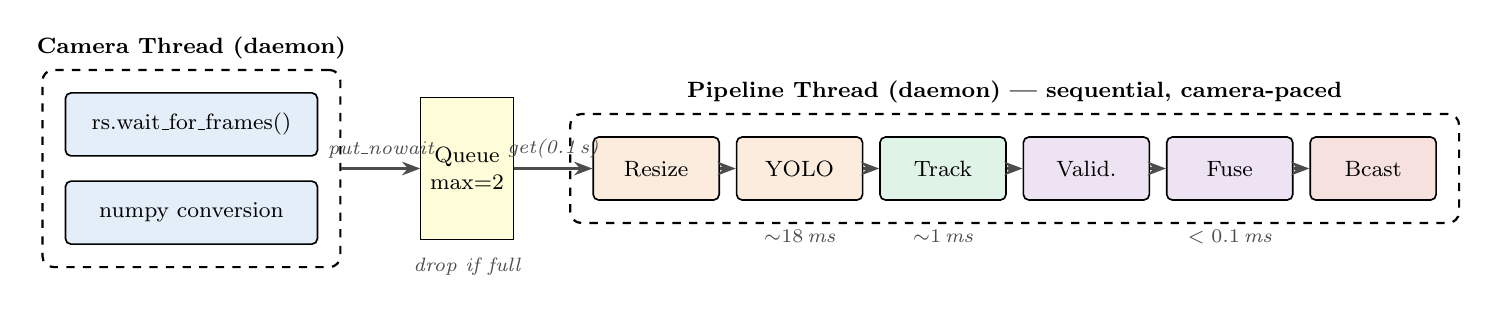
\begin{tikzpicture}[
    >=Stealth,
    node distance=0.4cm and 0.3cm,
    stage/.style={
      draw, rectangle, rounded corners=2pt,
      minimum height=0.8cm, align=center,
      font=\footnotesize, line width=0.6pt},
    thread/.style={
      draw, rectangle, rounded corners=4pt,
      inner sep=8pt, dashed, line width=0.8pt},
    qlabel/.style={
      font=\scriptsize\ttfamily, text=black},
    arr/.style={->, thick, color=black!70},
    anno/.style={font=\scriptsize\itshape, text=gray!60!black},
  ]

  % ── Capture thread ──
  \node[stage, fill=sensing!15, minimum width=3.2cm]
    (rs) {rs.wait\_for\_frames()};
  \node[stage, fill=sensing!15, minimum width=3.2cm, below=0.3cm of rs]
    (np) {numpy conversion};

  \node[thread, fit=(rs)(np), label={[font=\footnotesize\bfseries]
    above:Camera Thread (daemon)}] (thr1) {};

  % ── Queue ──
  \node[draw, rectangle, fill=yellow!15,
        minimum width=1.0cm, minimum height=1.8cm,
        right=1.0cm of thr1, font=\footnotesize, align=center]
    (q) {Queue\\max=2};
  \node[anno, below=0.1cm of q] {drop if full};

  \draw[arr] (thr1.east) -- (q.west)
    node[midway, above, anno] {put\_nowait};

  % ── Pipeline thread stages ──
  \node[stage, fill=vision!15,     right=1.0cm of q,
        minimum width=1.6cm] (s1) {Resize};
  \node[stage, fill=vision!15,     right=0.2cm of s1,
        minimum width=1.6cm] (s2) {YOLO};
  \node[stage, fill=estimation!15, right=0.2cm of s2,
        minimum width=1.6cm] (s3) {Track};
  \node[stage, fill=validation!15, right=0.2cm of s3,
        minimum width=1.6cm] (s4) {Valid.};
  \node[stage, fill=validation!15, right=0.2cm of s4,
        minimum width=1.6cm] (s5) {Fuse};
  \node[stage, fill=output!15,     right=0.2cm of s5,
        minimum width=1.6cm] (s6) {Bcast};

  % ── Fit pipeline thread ──
  \node[thread, fit=(s1)(s2)(s3)(s4)(s5)(s6),
    label={[font=\footnotesize\bfseries]
      above:Pipeline Thread (daemon) --- sequential, camera-paced}]
    (thr2) {};

  \draw[arr] (q.east) -- (s1.west)
    node[midway, above, anno] {get(0.1\,s)};
  \draw[arr] (s1) -- (s2);
  \draw[arr] (s2) -- (s3);
  \draw[arr] (s3) -- (s4);
  \draw[arr] (s4) -- (s5);
  \draw[arr] (s5) -- (s6);

  % ── Timing annotations ──
  \node[anno, below=0.25cm of s2] {${\sim}18$\,ms};
  \node[anno, below=0.25cm of s3] {${\sim}1$\,ms};
  \node[anno, below=0.25cm of s5] {$<0.1$\,ms};

\end{tikzpicture}
\caption{Threading model and per-stage timing budget.
         The pipeline thread executes all stages sequentially
         on each frame; frame pacing is governed by the camera
         hardware at 30\,fps.  Under overload, the bounded queue
         drops frames to preserve freshness.}
\label{fig:threading}
\end{figure}

\noindent
This architecture enforces a unidirectional data flow from sensing to
output, minimizing cross-module coupling and simplifying reasoning
about timing and correctness.  Each subsystem exposes a well-defined
interface, allowing alternative implementations---such as different
trackers or detectors---to be integrated without modifying the overall
pipeline structure.  The design targets real-time execution on embedded
hardware (NVIDIA Jetson Orin Nano) while maintaining extensibility for
experimentation and algorithmic upgrades.

\end{document}
